
%% bare_conf.tex
%% V1.3
%% 2007/01/11
%% by Michael Shell
%% See:
%% http://www.michaelshell.org/
%% for current contact information.
%%
%% This is a skeleton file demonstrating the use of IEEEtran.cls
%% (requires IEEEtran.cls version 1.7 or later) with an IEEE conference paper.
%%
%% Support sites:
%% http://www.michaelshell.org/tex/ieeetran/
%% http://www.ctan.org/tex-archive/macros/latex/contrib/IEEEtran/
%% and
%% http://www.ieee.org/

%%*************************************************************************
%% Legal Notice:
%% This code is offered as-is without any warranty either expressed or
%% implied; without even the implied warranty of MERCHANTABILITY or
%% FITNESS FOR A PARTICULAR PURPOSE! 
%% User assumes all risk.
%% In no event shall IEEE or any contributor to this code be liable for
%% any damages or losses, including, but not limited to, incidental,
%% consequential, or any other damages, resulting from the use or misuse
%% of any information contained here.
%%
%% All comments are the opinions of their respective authors and are not
%% necessarily endorsed by the IEEE.
%%
%% This work is distributed under the LaTeX Project Public License (LPPL)
%% ( http://www.latex-project.org/ ) version 1.3, and may be freely used,
%% distributed and modified. A copy of the LPPL, version 1.3, is included
%% in the base LaTeX documentation of all distributions of LaTeX released
%% 2003/12/01 or later.
%% Retain all contribution notices and credits.
%% ** Modified files should be clearly indicated as such, including  **
%% ** renaming them and changing author support contact information. **
%%
%% File list of work: IEEEtran.cls, IEEEtran_HOWTO.pdf, bare_adv.tex,
%%                    bare_conf.tex, bare_jrnl.tex, bare_jrnl_compsoc.tex
%%*************************************************************************

% *** Authors should verify (and, if needed, correct) their LaTeX system  ***
% *** with the testflow diagnostic prior to trusting their LaTeX platform ***
% *** with production work. IEEE's font choices can trigger bugs that do  ***
% *** not appear when using other class files.                            ***
% The testflow support page is at:
% http://www.michaelshell.org/tex/testflow/



% Note that the a4paper option is mainly intended so that authors in
% countries using A4 can easily print to A4 and see how their papers will
% look in print - the typesetting of the document will not typically be
% affected with changes in paper size (but the bottom and side margins will).
% Use the testflow package mentioned above to verify correct handling of
% both paper sizes by the user's LaTeX system.
%
% Also note that the "draftcls" or "draftclsnofoot", not "draft", option
% should be used if it is desired that the figures are to be displayed in
% draft mode.
%
\documentclass[conference]{IEEEtran}
\usepackage{blindtext, graphicx}
\usepackage{amsmath}
\usepackage{url}
\usepackage{float}
\usepackage{placeins} %for float barriers
\usepackage[table,xcdraw]{xcolor}
\usepackage{pgfplots}
\usepackage{titlesec}
\pgfplotsset{height = 7.5cm, width = 2.5in, compat=1.13}
\setlength{\textfloatsep}{-5pt plus 1.0pt minus 2.0pt}
\setlength{\intextsep}{5pt plus 1.0pt minus 2.0pt}
\titlespacing*{\section}{0pt}{0ex plus 1ex minus .2ex}{0ex plus .2ex}
\titlespacing*{\subsection}{0pt}{0ex plus 1ex minus .2ex}{0ex plus .2ex}
% Add the compsoc option for Computer Society conferences.
%
% If IEEEtran.cls has not been installed into the LaTeX system files,
% manually specify the path to it like:
% \documentclass[conference]{../sty/IEEEtran}





% Some very useful LaTeX packages include:
% (uncomment the ones you want to load)


% *** MISC UTILITY PACKAGES ***
%
%\usepackage{ifpdf}
% Heiko Oberdiek's ifpdf.sty is very useful if you need conditional
% compilation based on whether the output is pdf or dvi.
% usage:
% \ifpdf
%   % pdf code
% \else
%   % dvi code
% \fi
% The latest version of ifpdf.sty can be obtained from:
% http://www.ctan.org/tex-archive/macros/latex/contrib/oberdiek/
% Also, note that IEEEtran.cls V1.7 and later provides a builtin
% \ifCLASSINFOpdf conditional that works the same way.
% When switching from latex to pdflatex and vice-versa, the compiler may
% have to be run twice to clear warning/error messages.






% *** CITATION PACKAGES ***
%
%\usepackage{cite}
% cite.sty was written by Donald Arseneau
% V1.6 and later of IEEEtran pre-defines the format of the cite.sty package
% \cite{} output to follow that of IEEE. Loading the cite package will
% result in citation numbers being automatically sorted and properly
% "compressed/ranged". e.g., [1], [9], [2], [7], [5], [6] without using
% cite.sty will become [1], [2], [5]--[7], [9] using cite.sty. cite.sty's
% \cite will automatically add leading space, if needed. Use cite.sty's
% noadjust option (cite.sty V3.8 and later) if you want to turn this off.
% cite.sty is already installed on most LaTeX systems. Be sure and use
% version 4.0 (2003-05-27) and later if using hyperref.sty. cite.sty does
% not currently provide for hyperlinked citations.
% The latest version can be obtained at:
% http://www.ctan.org/tex-archive/macros/latex/contrib/cite/
% The documentation is contained in the cite.sty file itself.






% *** GRAPHICS RELATED PACKAGES ***
%
\ifCLASSINFOpdf
  % \usepackage[pdftex]{graphicx}
  % declare the path(s) where your graphic files are
  % \graphicspath{{../pdf/}{../jpeg/}}
  % and their extensions so you won't have to specify these with
  % every instance of \includegraphics
  % \DeclareGraphicsExtensions{.pdf,.jpeg,.png}
\else
  % or other class option (dvipsone, dvipdf, if not using dvips). graphicx
  % will default to the driver specified in the system graphics.cfg if no
  % driver is specified.
  % \usepackage[dvips]{graphicx}
  % declare the path(s) where your graphic files are
  % \graphicspath{{../eps/}}
  % and their extensions so you won't have to specify these with
  % every instance of \includegraphics
  % \DeclareGraphicsExtensions{.eps}
\fi
% graphicx was written by David Carlisle and Sebastian Rahtz. It is
% required if you want graphics, photos, etc. graphicx.sty is already
% installed on most LaTeX systems. The latest version and documentation can
% be obtained at: 
% http://www.ctan.org/tex-archive/macros/latex/required/graphics/
% Another good source of documentation is "Using Imported Graphics in
% LaTeX2e" by Keith Reckdahl which can be found as epslatex.ps or
% epslatex.pdf at: http://www.ctan.org/tex-archive/info/
%
% latex, and pdflatex in dvi mode, support graphics in encapsulated
% postscript (.eps) format. pdflatex in pdf mode supports graphics
% in .pdf, .jpeg, .png and .mps (metapost) formats. Users should ensure
% that all non-photo figures use a vector format (.eps, .pdf, .mps) and
% not a bitmapped formats (.jpeg, .png). IEEE frowns on bitmapped formats
% which can result in "jaggedy"/blurry rendering of lines and letters as
% well as large increases in file sizes.
%
% You can find documentation about the pdfTeX application at:
% http://www.tug.org/applications/pdftex





% *** MATH PACKAGES ***
%
%\usepackage[cmex10]{amsmath}
% A popular package from the American Mathematical Society that provides
% many useful and powerful commands for dealing with mathematics. If using
% it, be sure to load this package with the cmex10 option to ensure that
% only type 1 fonts will utilized at all point sizes. Without this option,
% it is possible that some math symbols, particularly those within
% footnotes, will be rendered in bitmap form which will result in a
% document that can not be IEEE Xplore compliant!
%
% Also, note that the amsmath package sets \interdisplaylinepenalty to 10000
% thus preventing page breaks from occurring within multiline equations. Use:
%\interdisplaylinepenalty=2500
% after loading amsmath to restore such page breaks as IEEEtran.cls normally
% does. amsmath.sty is already installed on most LaTeX systems. The latest
% version and documentation can be obtained at:
% http://www.ctan.org/tex-archive/macros/latex/required/amslatex/math/





% *** SPECIALIZED LIST PACKAGES ***
%
%\usepackage{algorithmic}
% algorithmic.sty was written by Peter Williams and Rogerio Brito.
% This package provides an algorithmic environment fo describing algorithms.
% You can use the algorithmic environment in-text or within a figure
% environment to provide for a floating algorithm. Do NOT use the algorithm
% floating environment provided by algorithm.sty (by the same authors) or
% algorithm2e.sty (by Christophe Fiorio) as IEEE does not use dedicated
% algorithm float types and packages that provide these will not provide
% correct IEEE style captions. The latest version and documentation of
% algorithmic.sty can be obtained at:
% http://www.ctan.org/tex-archive/macros/latex/contrib/algorithms/
% There is also a support site at:
% http://algorithms.berlios.de/index.html
% Also of interest may be the (relatively newer and more customizable)
% algorithmicx.sty package by Szasz Janos:
% http://www.ctan.org/tex-archive/macros/latex/contrib/algorithmicx/




% *** ALIGNMENT PACKAGES ***
%
%\usepackage{array}
% Frank Mittelbach's and David Carlisle's array.sty patches and improves
% the standard LaTeX2e array and tabular environments to provide better
% appearance and additional user controls. As the default LaTeX2e table
% generation code is lacking to the point of almost being broken with
% respect to the quality of the end results, all users are strongly
% advised to use an enhanced (at the very least that provided by array.sty)
% set of table tools. array.sty is already installed on most systems. The
% latest version and documentation can be obtained at:
% http://www.ctan.org/tex-archive/macros/latex/required/tools/


%\usepackage{mdwmath}
%\usepackage{mdwtab}
% Also highly recommended is Mark Wooding's extremely powerful MDW tools,
% especially mdwmath.sty and mdwtab.sty which are used to format equations
% and tables, respectively. The MDWtools set is already installed on most
% LaTeX systems. The lastest version and documentation is available at:
% http://www.ctan.org/tex-archive/macros/latex/contrib/mdwtools/


% IEEEtran contains the IEEEeqnarray family of commands that can be used to
% generate multiline equations as well as matrices, tables, etc., of high
% quality.


%\usepackage{eqparbox}
% Also of notable interest is Scott Pakin's eqparbox package for creating
% (automatically sized) equal width boxes - aka "natural width parboxes".
% Available at:
% http://www.ctan.org/tex-archive/macros/latex/contrib/eqparbox/





% *** SUBFIGURE PACKAGES ***
%\usepackage[tight,footnotesize]{subfigure}
% subfigure.sty was written by Steven Douglas Cochran. This package makes it
% easy to put subfigures in your figures. e.g., "Figure 1a and 1b". For IEEE
% work, it is a good idea to load it with the tight package option to reduce
% the amount of white space around the subfigures. subfigure.sty is already
% installed on most LaTeX systems. The latest version and documentation can
% be obtained at:
% http://www.ctan.org/tex-archive/obsolete/macros/latex/contrib/subfigure/
% subfigure.sty has been superceeded by subfig.sty.



\usepackage[caption=false]{caption}
\usepackage[font=footnotesize]{subfig}
% subfig.sty, also written by Steven Douglas Cochran, is the modern
% replacement for subfigure.sty. However, subfig.sty requires and
% automatically loads Axel Sommerfeldt's caption.sty which will override
% IEEEtran.cls handling of captions and this will result in nonIEEE style
% figure/table captions. To prevent this problem, be sure and preload
% caption.sty with its "caption=false" package option. This is will preserve
% IEEEtran.cls handing of captions. Version 1.3 (2005/06/28) and later 
% (recommended due to many improvements over 1.2) of subfig.sty supports
% the caption=false option directly:
%\usepackage[caption=false,font=footnotesize]{subfig}
%
% The latest version and documentation can be obtained at:
% http://www.ctan.org/tex-archive/macros/latex/contrib/subfig/
% The latest version and documentation of caption.sty can be obtained at:
% http://www.ctan.org/tex-archive/macros/latex/contrib/caption/




% *** FLOAT PACKAGES ***
%
%\usepackage{fixltx2e}
% fixltx2e, the successor to the earlier fix2col.sty, was written by
% Frank Mittelbach and David Carlisle. This package corrects a few problems
% in the LaTeX2e kernel, the most notable of which is that in current
% LaTeX2e releases, the ordering of single and double column floats is not
% guaranteed to be preserved. Thus, an unpatched LaTeX2e can allow a
% single column figure to be placed prior to an earlier double column
% figure. The latest version and documentation can be found at:
% http://www.ctan.org/tex-archive/macros/latex/base/



%\usepackage{stfloats}
% stfloats.sty was written by Sigitas Tolusis. This package gives LaTeX2e
% the ability to do double column floats at the bottom of the page as well
% as the top. (e.g., "\begin{figure*}[!b]" is not normally possible in
% LaTeX2e). It also provides a command:
%\fnbelowfloat
% to enable the placement of footnotes below bottom floats (the standard
% LaTeX2e kernel puts them above bottom floats). This is an invasive package
% which rewrites many portions of the LaTeX2e float routines. It may not work
% with other packages that modify the LaTeX2e float routines. The latest
% version and documentation can be obtained at:
% http://www.ctan.org/tex-archive/macros/latex/contrib/sttools/
% Documentation is contained in the stfloats.sty comments as well as in the
% presfull.pdf file. Do not use the stfloats baselinefloat ability as IEEE
% does not allow \baselineskip to stretch. Authors submitting work to the
% IEEE should note that IEEE rarely uses double column equations and
% that authors should try to avoid such use. Do not be tempted to use the
% cuted.sty or midfloat.sty packages (also by Sigitas Tolusis) as IEEE does
% not format its papers in such ways.





% *** PDF, URL AND HYPERLINK PACKAGES ***
%
%\usepackage{url}
% url.sty was written by Donald Arseneau. It provides better support for
% handling and breaking URLs. url.sty is already installed on most LaTeX
% systems. The latest version can be obtained at:
% http://www.ctan.org/tex-archive/macros/latex/contrib/misc/
% Read the url.sty source comments for usage information. Basically,
% \url{my_url_here}.





% *** Do not adjust lengths that control margins, column widths, etc. ***
% *** Do not use packages that alter fonts (such as pslatex).         ***
% There should be no need to do such things with IEEEtran.cls V1.6 and later.
% (Unless specifically asked to do so by the journal or conference you plan
% to submit to, of course. )


% correct bad hyphenation here
\hyphenation{op-tical net-works semi-conduc-tor}


\begin{document}
%
% paper title
% can use linebreaks \\ within to get better formatting as desired
\title{Implementation and Testing of an (8, 4, 4) Viterbi Decoder}


% author names and affiliations
% use a multiple column layout for up to three different
% affiliations
\author{\IEEEauthorblockN{Harsh Aurora}
\IEEEauthorblockA{260394216\\
harsh.aurora@mail.mcgill.ca}
\and
\IEEEauthorblockN{Adam Cavatassi}
\IEEEauthorblockA{260409261\\
adam.cavatassi@mail.mcgill.ca}
\and 
\IEEEauthorblockN{Xiaoqing Ma}
\IEEEauthorblockA{260668927\\
xiaoqing.ma@mail.mcgill.ca}

\and
\IEEEauthorblockN{Dylan Watts}
\IEEEauthorblockA{260406792\\
dylan.watts@mail.mcgill.ca}}
% conference papers do not typically use \thanks and this command
% is locked out in conference mode. If really needed, such as for
% the acknowledgment of grants, issue a \IEEEoverridecommandlockouts
% after \documentclass

% for over three affiliations, or if they all won't fit within the width
% of the page, use this alternative format:
% 
%\author{\IEEEauthorblockN{Michael Shell\IEEEauthorrefmark{1},
%Homer Simpson\IEEEauthorrefmark{2},
%James Kirk\IEEEauthorrefmark{3}, 
%Montgomery Scott\IEEEauthorrefmark{3} and
%Eldon Tyrell\IEEEauthorrefmark{4}}
%\IEEEauthorblockA{\IEEEauthorrefmark{1}School of Electrical and Computer Engineering\\
%Georgia Institute of Technology,
%Atlanta, Georgia 30332--0250\\ Email: see http://www.michaelshell.org/contact.html}
%\IEEEauthorblockA{\IEEEauthorrefmark{2}Twentieth Century Fox, Springfield, USA\\
%Email: homer@thesimpsons.com}
%\IEEEauthorblockA{\IEEEauthorrefmark{3}Starfleet Academy, San Francisco, California 96678-2391\\
%Telephone: (800) 555--1212, Fax: (888) 555--1212}
%\IEEEauthorblockA{\IEEEauthorrefmark{4}Tyrell Inc., 123 Replicant Street, Los Angeles, California 90210--4321}}




% use for special paper notices
%\IEEEspecialpapernotice{(Invited Paper)}




% make the title area
\maketitle


\begin{abstract}
%\boldmath
This paper presents the basic knowledge and circuit design for an (8, 4, 4) Viterbi decoder. Two different designs are given to optimize either computation speed or power consumption. The decoder architecture is verified by logic simulation in Modelsim with Verilog. Timing analysis and circuit simulation in IRSIM and SPICE are done to find the computation delay and the amount of power consumed for both designs. The repository and \LaTeX\  code for this report can be accessed by visiting: \url{https://github.com/xiaoqing1993/ECSE548_viterbi_decoder}

\end{abstract}
% IEEEtran.cls defaults to using nonbold math in the Abstract.
% This preserves the distinction between vectors and scalars. However,
% if the journal you are submitting to favors bold math in the abstract,
% then you can use LaTeX's standard command \boldmath at the very start
% of the abstract to achieve this. Many IEEE journals frown on math
% in the abstract anyway.

% Note that keywords are not normally used for peerreview papers.
%\begin{IEEEkeywords}
%IEEEtran, journal, \LaTeX, paper, template.
%\end{IEEEkeywords}






% For peer review papers, you can put extra information on the cover
% page as needed:
% \ifCLASSOPTIONpeerreview
% \begin{center} \bfseries EDICS Category: 3-BBND \end{center}
% \fi
%
% For peerreview papers, this IEEEtran command inserts a page break and
% creates the second title. It will be ignored for other modes.
\IEEEpeerreviewmaketitle



\section{Introduction}
For this project, our goal is to design two different circuits of an (8, 4, 4) Viterbi decoder for different purpose: one is power-efficient while the other runs in a high speed. To eliminate the power consumption, carry-ripple adders are implemented in the first design. In another design, Kogge-Stone adders are introduced to speed up the computation. The schematic and layout designs for all modules and the overall decoder are finished in electric.

Simulation process of this project can be divided into two parts. The first part is logic verification, which has been conducted with Verilog using Modelsim. The second part is circuit simulation for finding delays and power consumptions. This work has been done within MATLAB, IRSIM and LTSPICE.

This report is organized as follow: Section II introduces the background knowledge of Viterbi decoder and section III presents the schematics and layouts of related modules and the overall decoder. Simulation procedures and results are presented in Section IV and V. Conclusions are drawn in Section VI.

\section {Background}
Error correction codes are employed to counter the effects of the noise introduced by the channel in data transmission. One such coding scheme is the Hamming (8,4,4) code, which is a systematic parity check code in which 4 message bits are used to produce an 8 bit codeword. The first four bits of the codeword are the message bits themselves (systematic), while the remaining four bits (parities) are calculated through XOR operations on the message bits three at a time. The numbers in (8,4,4) then represent the codeword length (8 bits), the number of information bits (4 bits), and the minimum distance of the code (4), which is a parameter that is used to describe the error correction capability of the code. The Hamming (8,4,4) code is constructed using the equations shown below.
\begin{equation}
\begin{align}
    \text{Message:}\ &m_{0}m_{1}m_{2}m_{3}\\
    \text{Codeword:}\ &c_{0} = m_{0}\ c_{1} = m_{1}\ c_{2} = m_{2}\ c_{3} = m_{3}\\
    &c_{4} = m_{0}\oplus m_{1}\oplus m_{2}\\
    &c_{5} = m_{0}\oplus m_{1}\oplus m_{3}\\
    &c_{6} = m_{0}\oplus m_{2}\oplus m_{3}\\
    &c_{7} = m_{1}\oplus m_{2}\oplus m_{3}\\
\end{align}
\end{equation}
Like all parity check codes, the Hamming (8,4,4) code can also be described using the Generator matrix G for the code.
\begin{equation}
\begin{align}
G&=
\begin{bmatrix}
1 & 0 & 0 & 0 & 1 & 1 & 1 & 0\\ 
0 & 1 & 0 & 0 & 1 & 1 & 0 & 1\\ 
0 & 0 & 1 & 0 & 1 & 0 & 1 & 1\\ 
0 & 0 & 0 & 1 & 0 & 1 & 1 & 1
\end{bmatrix}\\
\vec{c} &= \vec{m}G
\end{align}
\end{equation}
Finally, another encoding scheme more suited for hardware is the optimized Trellis of the code shown in Figure \ref{fig:trellis}. This can be implemented as a state machine in which the four message bits that are passed in as an input traverse a unique path in the Trellis, through which the codeword can be extracted. 
\begin{figure}[h!]
\centering
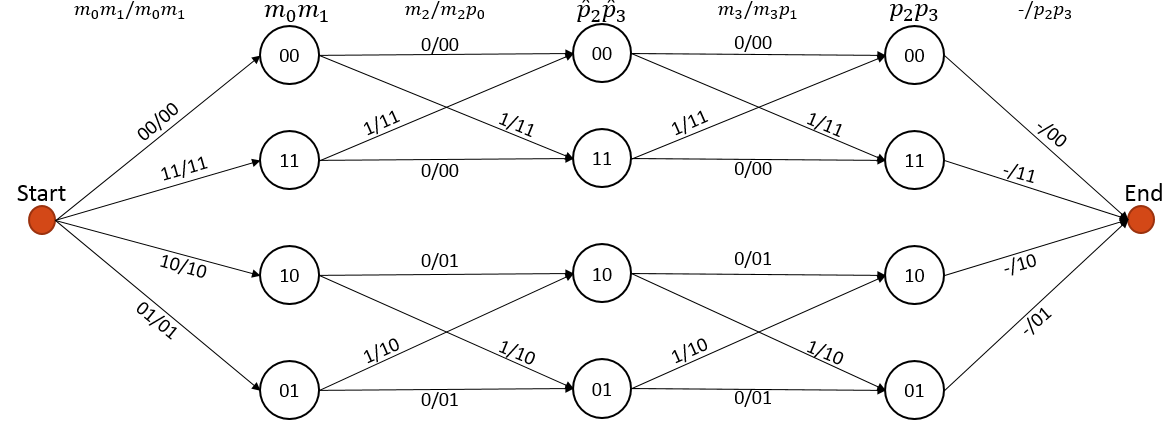
\includegraphics[scale=0.3]{trellis}
\caption{Encoding Trellis for (8, 4, 4) Hamming Code}
\label{fig:trellis}
\end{figure}

To transmit the codeword in a channel, a certain modulation scheme is necessary. Here we use BPSK modulation, which modulates binary 0 to -0.5 and 1 to 0.5. Using this modulation scheme, codeword $\vec{c}$ is modulated to the channel input $\vec{x}$. During transmission, signals are subject to corruption by noise, which can be characterized by signal-noise-ratio(SNR). The equation for computing SNR is shown below, where $E_{b}$ denotes the energy per bit and $N_{o}$ denotes the noise spectral density. 
\begin{equation}
SNR = \frac{E_{b}}{N_{o}} (dB)
\end{equation}
A noise vector $\vec{n}=n_{0}n_{1}n_{2}n_{3}n_{4}n_{5}n_{6}n_{7}$ can be generated from a zero-mean Gaussian distribution. By changing the variance of this Gaussian distribution, different SNR can be achieved. Since the Gaussian noise is additive, the channel observation $\vec{r}$ is computed as: 
\begin{equation}
\vec{r}=\vec{x}+\vec{n}
\end{equation}

The optimum decoding performance of the Hamming (8,4,4) code is achieved under Maximum Likelihood (MLE) decoding. This involves generating the entire codebook consisting of 16 codewords (one for each possible 4 bit message combination), and then calculating the distance between the received noisy channel observation and each codeword in the code book. The most likely transmitted codeword is then the one with the minimum distance to the channel output. This approach is computationally intensive, however, both in space and time. Coming back to the Trellis of the code, it can be observed that the noisy channel observation can be used in conjunction with the Viterbi algorithm to calculate the most likely path traversed along the Trellis, and hence the most likely transmitted codeword. Incorporating the modulation scheme and taking advantage of the symmetricity of the Trellis can further reduce the number of computations, and most notably eliminate the need for any multiplications. The entire decoding process can then be carried out using only 18 additions and 11 comparisons. This decoding approach is theoretically expected and verified through simulation to have the exact same decoding performance as the MLE decoder.

In the decoder, fixed point arithmetic are used to compute floating point operations. The fixed point format Qn.m represents a floating point number $f$ as an $(n+m)$ bits binary number. The representation process can be shown as in the equation below:
\begin{equation}
\begin{align*}
f = &-2^{n-1}b_{n-1}+2^{n-2}b_{n-2}+...\\
&+2^{0}b_{0}+2^{-1}b_{-1}+...+2^{-m}b_{-m}
\end{align*}
\end{equation}

Fixed point arithmetic is implemented in the same manner as 2`s complement arithmetic with the exception that an overflow/underflow is handled by saturating the result at the maximum/minimum value of the Qn.m format. The performance of the Viterbi decoder for different Qn.m formats are shown in Figure \ref{fig:qnm}.
\begin{figure}[h!]
\centering
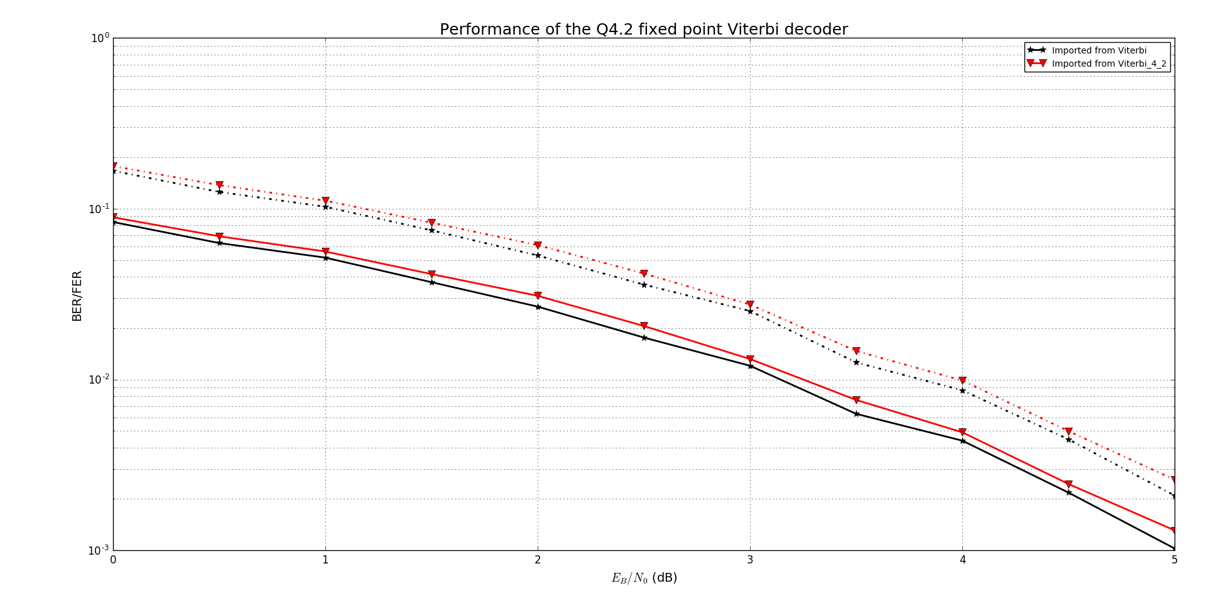
\includegraphics[scale=0.4]{qnm}
\caption{Performance of various fixed point lengths}
\label{fig:qnm}
\end{figure}

For Q3.10, the bits for integer are too few to provide an enough range. However for Q6.2, the improvement from larger integer range is limited. Therefore 4 bits for integer can be satisfactory. Q4.10 can provide a much more precise representation, but the cost is high. Despite slight quantization noise, Q4.2 is a good choice to be implemented.
\section{Circuit Design}
In the circuit design of this project, we will target the AMI 0.5 μm process using the MOSIS scalable CMOS submicron design rules with λ = 0.3 μm. This is the same design rule with labs from this course. In order to compare the performances of different designs, we present two kinds of schematics and layouts of the Viterbi decoder, each of which is optimized for power or speed respectively.

As we are using a data structure of 6 bits, a Viterbi decoder can be made up of several 6-bit adders, comparators and multiplexers. Schematics and layouts of these required modules and the overall decoder circuit designed in electric will be presented in the following part of this section.

\subsection{Adder}
Optimization methods for speed and power are different from each other in the choices of 6-bit adders. Carry-ripple adders are chosen for the power-efficient design, while Kogge-stone adders are selected to achieve fast computation for the other.

Also, further modifications should be made to adjust an ordinary adder to a fixed point adder. Fixed point notation can be added and subtracted the same way that signed binary is, but overflow needs to be handled differently. In a 6-bit signed number, possible values range from -32 to 31. The modified adder needs to assert the output to -32 when it detects overflow of the low range, and it needs to assert the output to 31 when overflow in the high range is detected. Let $a$ and $b$ be the two inputs of an adder. $y$ denotes the final output. The addition performed by a 6-bit fixed point adder can be expressed as a function in equation below: 
\begin{equation}
y=
\begin{cases}
-32\ (10000) & a+b<-32\\
a+b& -32\leq a+b < 31\\
31\ (01111)& a+b\geq 31\\
\end{cases}
\end{equation}
The determination of whether the sum of $a$ and $b$ is located in the range of $[-32, 31]$ can be made by comparing the most significant bit of one of operands and the output for a difference in sign. This subsection is going to introduce carry-ripple and kogge-stone adders as well as their modification approaches respectively.

\subsubsection{Carry-ripple adder (CRA)}

The basic carry-ripple adder is built from six single-bit full adders with their carry-in and carry-out ports connected. Additionally one XOR gate is needed to generate the overflow signal. The schematic and layout of the basic carry-ripple adder is shown in Figure \ref{fig:fulladder6}.
\begin{figure}[h]
\centerline{\subfloat[Schematic]{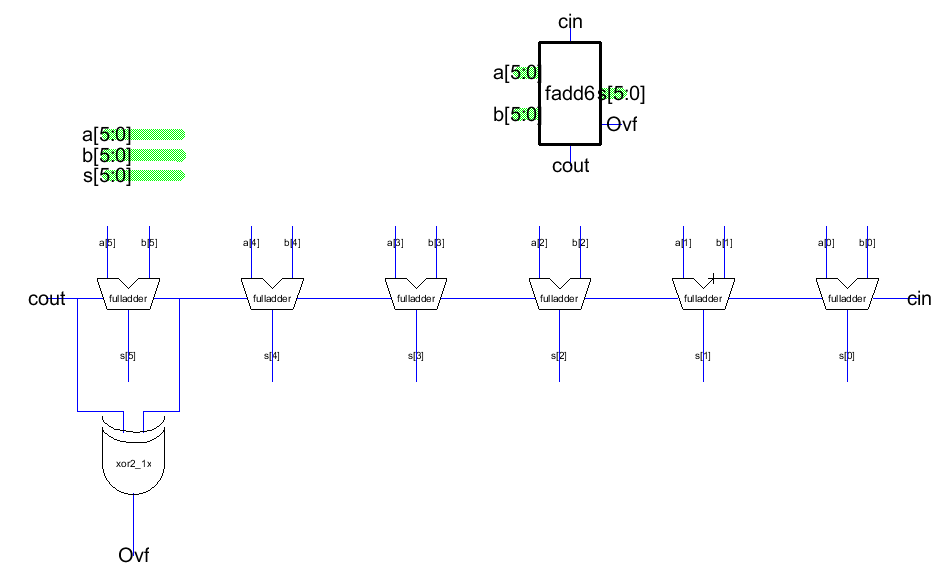
\includegraphics[scale=0.2]{fulladder6_sch}
\label{fig_first_case}}
\hfil
\subfloat[Layout]{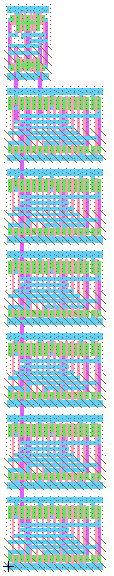
\includegraphics[scale=0.25]{fulladder6_lay}
\label{fig_second_case}}}
\caption{Circuit Design for 6-bit Full Adder}
\label{fig:fulladder6}
\end{figure}
The fixed point adder consists of the basic CRA and two 6-bit multiplexers. Multiplexers take advantage of the sign bit and overflow from the sum of inputs to select the proper output. Figure \ref{fig:cradder6} shows the schematic and layout of a CRA used in viterbi decoder.
\begin{figure}[h]
\centerline{\subfloat[Schematic]{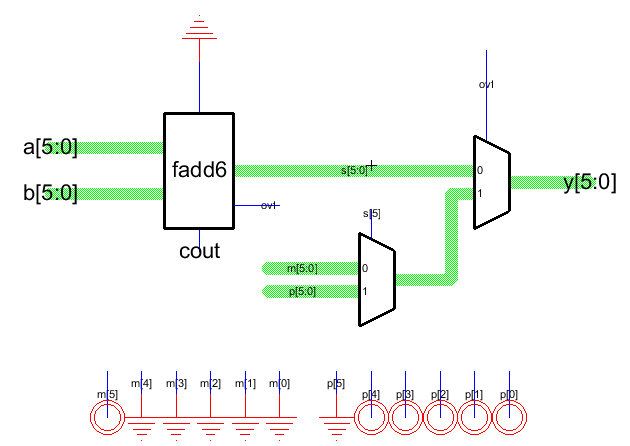
\includegraphics[scale=0.2]{adder6_sch2}
\label{fig_first_case}}
\hfil
\subfloat[Layout]{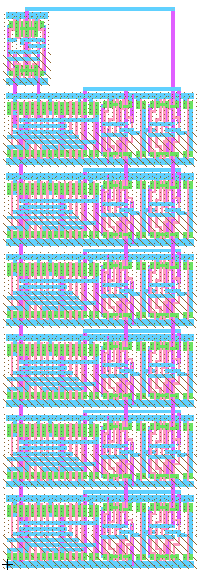
\includegraphics[scale=0.2]{adder6_lay}
\label{fig_second_case}}}
\caption{Circuit Design for Fixed Point 6-bit Carry-Ripple Adder}
\label{fig:cradder6}
\end{figure}

\subsubsection{Kogge-Stone adder (KSA)}
The Kogge-Stone adder is a tree adder that uses a specific design of carry-propagate layering. The benefit of this is that it computes carry signals in parallel, in contrast to the ripple carry adder. The ripple carry adder is comprised of a string of a full adder blocks. Each full adder block must wait for the carry out from the previous full adder before it can compute its own carry out. With large number of bits, this becomes a very slow method of addition. Our Kogge-Stone adder is made up of three basic logic blocks. One that computes propagate and generate from the operands, one that computes propagate and generate based on the previous level of propagate and generate, and one that computes only generate from the previous level. Schematics and layouts of these blocks can be found in the Electric file of this project. These blocks are wired together in a way that significantly reduces the critical path of the addition. The schematic and layout of this adder is shown in Figure \ref{fig:ksadder6_wm}.
\begin{figure}[h]
\centerline{\subfloat[Schematic]{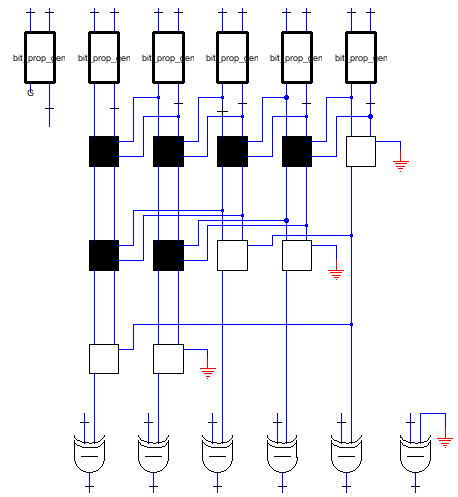
\includegraphics[scale=0.2]{ksa2}
\label{fig_first_case}}
\hfil
\subfloat[Layout]{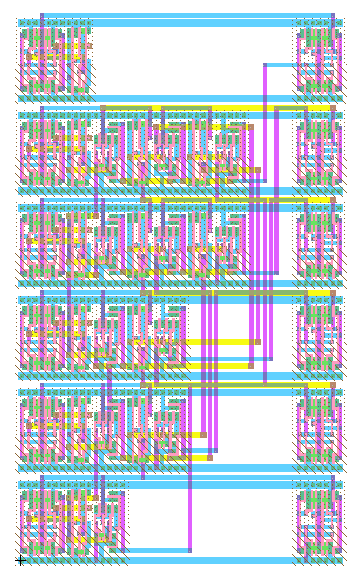
\includegraphics[scale=0.2]{ksa_lay}
\label{fig_second_case}}}
\caption{Circuit Design for 6-bit Kogge-Stone Adder}
\label{fig:ksadder6_wm}
\end{figure}

The Kogge-Stone adder operates only typical binary addition. The Viterbi design envisioned uses fixed point arithmetic. The Kogge-Stone adder can be modified to handle fixed point notation.The assertion of -32 or 31 can be done using six bit multiplexers that use the overflow signal as the selector. Once the multiplexer and overflow detection are appended, the Kogge-Stone adder is now a fixed point Kogge-Stone adder. Figure \ref{fig:ksadder6} presents the schematic and layout of the fixed point Kogge-Stone adder
\begin{figure}[h]
\centerline{\subfloat[Schematic]{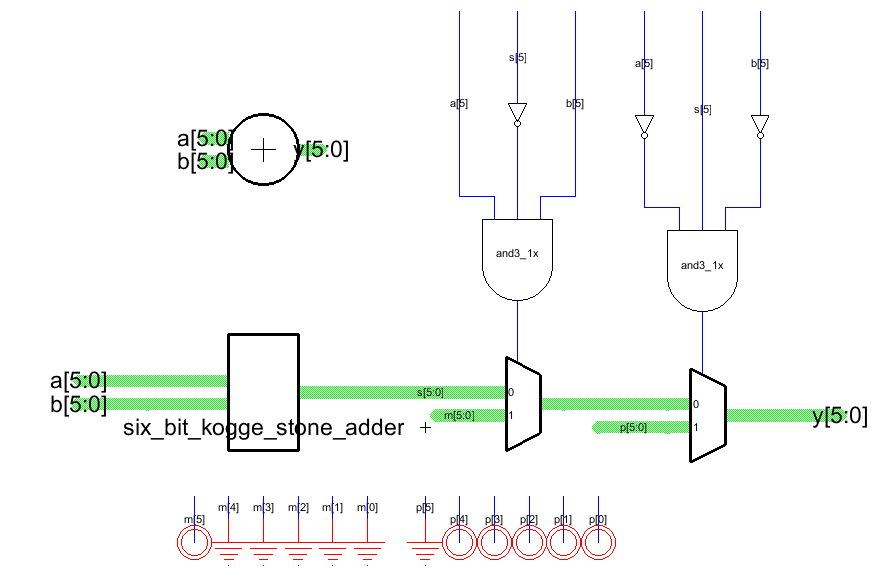
\includegraphics[scale=0.2]{adder6_ksa_sch}
\label{fig_first_case}}
\hfil
\subfloat[Layout]{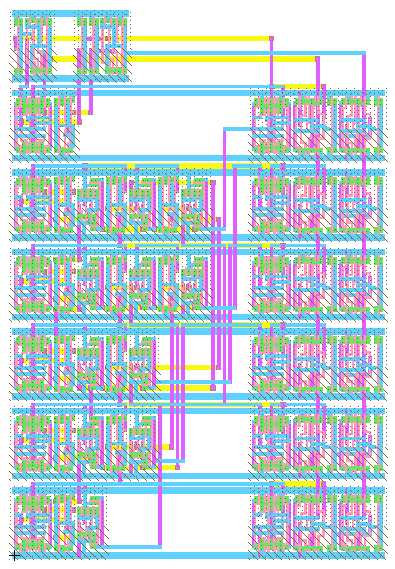
\includegraphics[scale=0.2]{adder6_ksa_lay}
\label{fig_second_case}}}
\caption{Circuit Design for Fixed Point 6-bit Kogge-Stone Adder}
\label{fig:ksadder6}
\end{figure}

There may be doubts as to whether or not the benefits of a Kogge-Stone adder can be realized with only six bits. As it stands, six bit addition requires five stages of propagation delay in the critical path of a ripple carry adder, while the critical path of a six bit Kogge-Stone adder is forced through only three stages. This 40\% reduction in stages could still present an increase in speed over the ripple carry adder, architecturally speaking. However, the Kogge-Stone adder is far more complex. It uses many more logic blocks, which means it consumes more power and it has more capacitance from its abundance of wires.

\subsection{Comparator}
The comparison of two 2`s complement binary numbers $a$ and $b$ can be done by computing $a-b$ and then determining whether the result is positive or negative by observing the result sign bit and overflow. Therefore to build a comparator, a 6-bit inverter, which is constructed with 6 single inverters from the standard cell library, and a 6-bit full adder from the previous CRA subsection are combined to compute subtraction, while an XOR gate is used to output the comparison decision. The schematic and layout of this 6-bit comparator can be found in the Electric file.
\subsection{Multiplexer}
Multiplexers are used to select the proper signal transmitting from the current stage to the next stage of a Viterbi decoder. In this project, a 6-bit multiplexer consists of 6 single-bit multiplexers from the standard cell library with their input nodes for selection connected together. The schematic and layout of this multiplexer can be found in the Electric file.
\subsection{Overall Decoder Design}
To decode an (8, 4, 4) Hamming code, the required numbers of each module are listed in table \ref{table:decoder} below
\begin{table}[h]
\centering
\caption{Required Number of Individual Modules}
\label{table:decoder}
\begin{tabular}{|c|c|}
\hline
Module                 & Required number \\ \hline
6-bit Adder            & 18              \\ \hline
6-bit Comparator       & 11              \\ \hline
6-bit Multiplexer      & 10              \\ \hline
Single-bit Multiplexer & 12              \\ \hline
Single-bit Inverter    & 6               \\ \hline
\end{tabular}
\end{table}

Figure \ref{fig:decoder_sch} presents the general schematic of a Viterbi decoder assembled from modules we discussed above. Figure \ref{fig:decoder_lay} shows the layout of the two decoders with carry-ripple adders and kogge-stone adders respectively. Both the layouts passed DRC, ERC and NCC successfully. 
\begin{figure}[h]
\centering
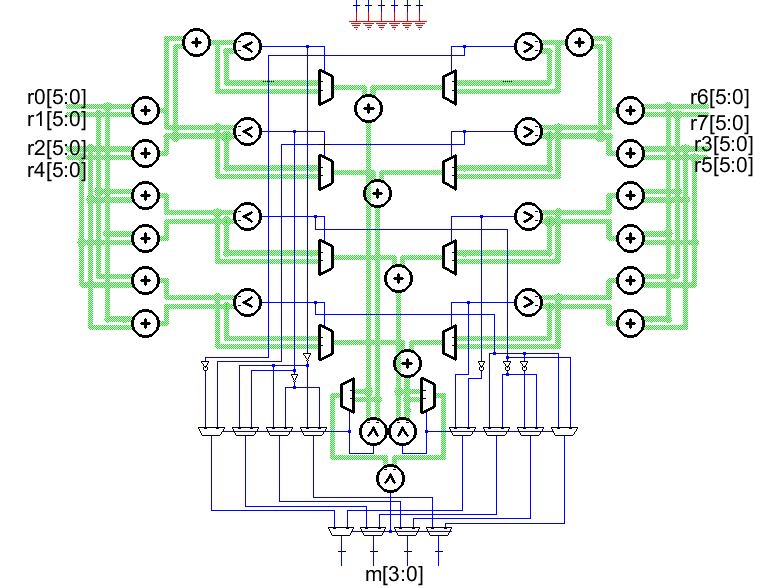
\includegraphics[scale=0.4]{decoder_sch}
\caption{Schematic of an (8, 4, 4) Viterbi Decoder}
\label{fig:decoder_sch}
\end{figure}
\begin{figure}[h]
\centerline{\subfloat[Decoder with CRA]{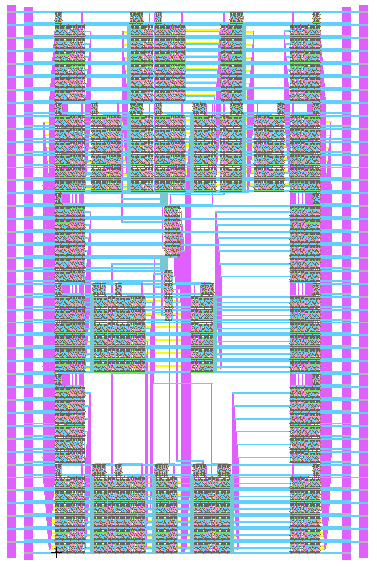
\includegraphics[scale=0.25]{decoder1_layout}
\label{fig_first_case}}
\hfil
\subfloat[Decoder with KSA]{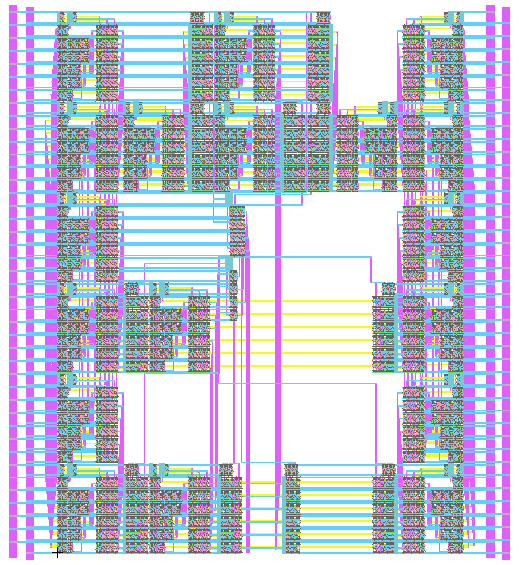
\includegraphics[scale=0.25]{decoder_ksa_layout}
\label{fig_second_case}}}
\caption{Layouts of 2 Viterbi Decoders}
\label{fig:decoder_lay}
\end{figure}
% needed in second column of first page if using \IEEEpubid
%\IEEEpubidadjcol

% An example of a floating figure using the graphicx package.
% Note that \label must occur AFTER (or within) \caption.
% For figures, \caption should occur after the \includegraphics.
% Note that IEEEtran v1.7 and later has special internal code that
% is designed to preserve the operation of \label within \caption
% even when the captionsoff option is in effect. However, because
% of issues like this, it may be the safest practice to put all your
% \label just after \caption rather than within \caption{}.
%
% Reminder: the "draftcls" or "draftclsnofoot", not "draft", class
% option should be used if it is desired that the figures are to be
% displayed while in draft mode.
%
%\begin{figure}[!t]
%\centering
%\includegraphics[width=2.5in]{myfigure}
% where an .eps filename suffix will be assumed under latex, 
% and a .pdf suffix will be assumed for pdflatex; or what has been declared
% via \DeclareGraphicsExtensions.
%\caption{Simulation Results}
%\label{fig_sim}
%\end{figure}

% Note that IEEE typically puts floats only at the top, even when this
% results in a large percentage of a column being occupied by floats.


% An example of a double column floating figure using two subfigures.
% (The subfig.sty package must be loaded for this to work.)
% The subfigure \label commands are set within each subfloat command, the
% \label for the overall figure must come after \caption.
% \hfil must be used as a separator to get equal spacing.
% The subfigure.sty package works much the same way, except \subfigure is
% used instead of \subfloat.
%
%\begin{figure*}[!t]
%\centerline{\subfloat[Case I]\includegraphics[width=2.5in]{subfigcase1}%
%\label{fig_first_case}}
%\hfil
%\subfloat[Case II]{\includegraphics[width=2.5in]{subfigcase2}%
%\label{fig_second_case}}}
%\caption{Simulation results}
%\label{fig_sim}
%\end{figure*}
%
% Note that often IEEE papers with subfigures do not employ subfigure
% captions (using the optional argument to \subfloat), but instead will
% reference/describe all of them (a), (b), etc., within the main caption.


% An example of a floating table. Note that, for IEEE style tables, the 
% \caption command should come BEFORE the table. Table text will default to
% \footnotesize as IEEE normally uses this smaller font for tables.
% The \label must come after \caption as always.
%
%\begin{table}[!t]
%% increase table row spacing, adjust to taste
%\renewcommand{\arraystretch}{1.3}
% if using array.sty, it might be a good idea to tweak the value of
% \extrarowheight as needed to properly center the text within the cells
%\caption{An Example of a Table}
%\label{table_example}
%\centering
%% Some packages, such as MDW tools, offer better commands for making tables
%% than the plain LaTeX2e tabular which is used here.
%\begin{tabular}{|c||c|}
%\hline
%One & Two\\
%\hline
%Three & Four\\
%\hline
%\end{tabular}
%\end{table}


% Note that IEEE does not put floats in the very first column - or typically
% anywhere on the first page for that matter. Also, in-text middle ("here")
% positioning is not used. Most IEEE journals use top floats exclusively.
% Note that, LaTeX2e, unlike IEEE journals, places footnotes above bottom
% floats. This can be corrected via the \fnbelowfloat command of the
% stfloats package.


\section{Logic Verification}
\subsection{Modelsim}
Most work of logic verification has been done in Modelsim. A fixed point Viterbi decoder has been created in verilog using ideal hardware modules. Noisy channel observations in Q4.2 format and expected decoder outputs are generated from C code. Using data extracted from C, a testbench can be built up around the Viterbi decoder. To test whether the hardware modules designed in Electric could function well, the ideal components in verilog programme can be substituted with the testing decks of every individual modules generated by Electric. One example of successful simulation in Modelsim is shown in Figure \ref{fig:modelsim}.
\begin{figure}[h]
\centering
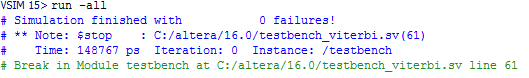
\includegraphics[scale=0.4]{decoder1_lay_sim}
\caption{An Example of Successful Simulation in Modelsim}
\label{fig:modelsim}
\end{figure}
\subsection{Electric}
Two decoder hardwares designed in Electric both passed DRC, ERC and NCC. Figure \ref{fig:electric} shows the screenshots of two decoder layouts passing all design checks.
\begin{figure}[h]
\centerline{\subfloat[Decoder with CRA]{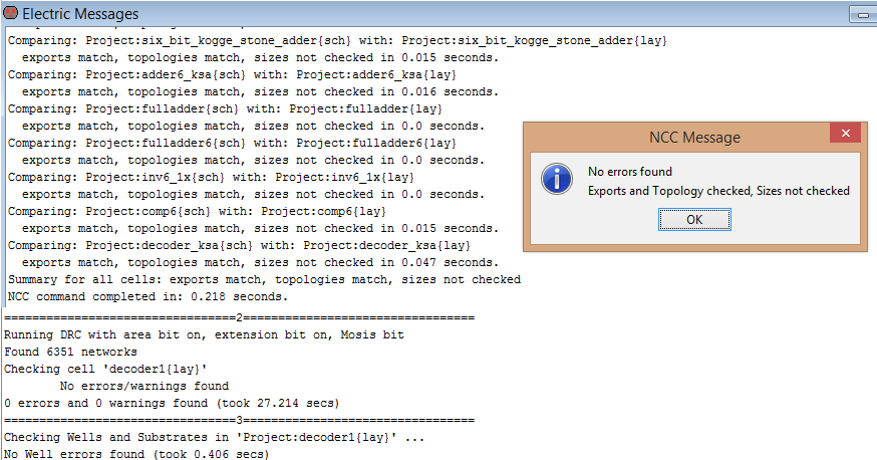
\includegraphics[scale=0.25]{drc_1}
\label{fig_first_case}}
\hfil
\subfloat[Decoder with KSA]{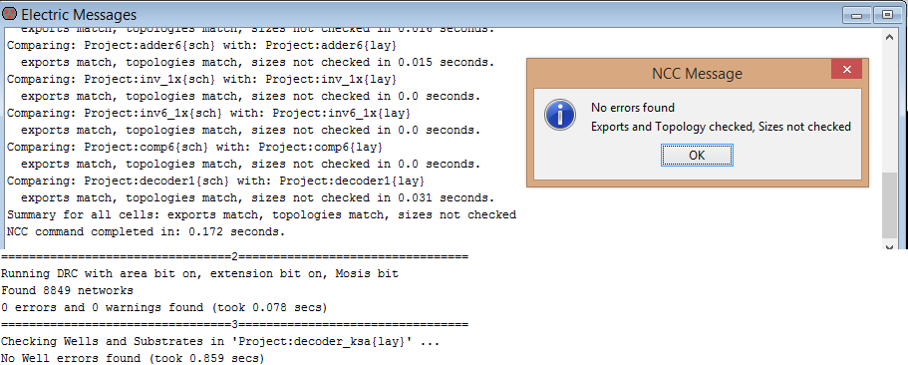
\includegraphics[scale=0.25]{drc_2}
\label{fig_second_case}}}
\caption{Demonstration of passing design checks}
\label{fig:electric}
\end{figure}
\section{Circuit Simulation}
\subsection{Testing Methodology}
While the circuit itself is not overly complicated, it requires 48 inputs leading to approximately 281 trillion input combinations. It is obvious that this is unfeasible to verify exhaustively, therefore a bounding approach must be adopted instead. To solve the issue of too many inputs, individual modules which makeup the top level will be individually tested. The maximum of which contains 12 inputs, or 4096 possible input combinations – a reasonable number for exhaustive testing. Bounds can then be obtained for each of these modules, and by multiplying these bounds by the number of modules contained in the top level an approximation can be obtained for the overall circuit.

\subsubsection{Capacitive Loading}
As each circuit is being tested in isolation, we must compensate for the absence of load by including a “characteristic capacitance” which mimics the load a circuit would drive if integrated into the overall circuit. If interconnect is neglected (as it is in the case of this report) the loading of a module consists of the output capacitance of the module and the input capacitance of the module to which it is connected. Since the output capacitance is accounted for during SPICE simulation, the remaining load can be characterised by adding a capacitor representative of the weighted average of the input capacitance of all modules in the circuit. There is also interest in the worst-case loading, which can be evaluated by substituting the average with the largest input capacitance of each module. The values of these characteristic capacitances are summarized below in Table \ref{tab:capacitance}.

\FloatBarrier
% Capacitance
\begin{table}[H]
\centering
\caption{Characteristic capacitance for various loading conditions.}
\label{tab:capacitance}
    \begin{tabular}{r|cc|}
    \cline{2-3}
    \multicolumn{1}{l|}{\cellcolor[HTML]{9B9B9B}{\color[HTML]{9B9B9B} }} & \multicolumn{1}{l|}{\textbf{Kogge-Stone}} & \multicolumn{1}{l|}{\textbf{Ripple Carry}} \\ \hline
    \multicolumn{1}{|r|}{\textbf{Avg Input Load (fF)}}                   & 38.59                                     & 36.53                                      \\ \cline{1-1}
    \multicolumn{1}{|r|}{\textbf{Max Input Load (fF)}}                   & 75.01                                     & 68.69                                      \\ \hline
    \end{tabular}
\end{table}
\FloatBarrier

\subsubsection{Power Consumption}


Our goal is to determine the average and worst case power consumption for each top-level module under various loading conditions. This can be accomplished by exhaustively simulating all possible switching conditions on LTSPICE and observing power consumption on a per-case basis. By multiplying the power statistics by the total number of modules in each decoder, we can get an idea of the average consumption and a conservative upper bound estimate, as it is assumed the probability that every module will be switching at its worst case is exceedingly rare.


\subsubsection{Propagation Delay}
There are two main simulations of propagation delay: dynamic and static. As dynamic delay represents the delay associated with each input vector, it is unfeasible to calculate for similar reasons as dynamic power consumption. Analysis will instead focus on static delay, which is characterised by converting the circuit into an edge/node weighted graph with weights representing interconnect/gate delay respectively.

In practice, static propagation delay is determined by inputting predetermined minimum and maximum standard cell delays into sophisticated circuit simulators. These would progress up through the circuit hierarchy, calculating delay at each step until an approximation is reached at the top level.  A similar methodology was employed in this report, however as these tools were unavailable various simplifying assumptions had to be made to allow calculation by hand (elaborated on in the following section). 

IRSIM was used to characterise min/max delay of basic gates, which were substituted into visually determined longest and shortest paths. This provided the propagation delay for each module at the lowest hierarchy level. To obtain the next level the process was iterated, substituting the values of the gates for the next level of the hierarchy, and so on until the system is fully characterised. As in power consumption interconnect was neglected, and the impact of this will be discussed in the Results section.


\subsection{Assumptions}
Due to the lack of sophisticated modelling software, several simplifying assumptions were required to allow for basic calculation. Much of these assumptions have the effect of producing a more conservative result, and those that do not will be discussed in detail in the Discussion section
\begin{itemize}
\setlength\itemsep{0.5em}
  \item Assume uniform distribution of input vectors – not true in general, but conservative.
  \item Neglect static power dissipation due to size of process, assume switching power is dominant factor.
  \item Delay of all outputs equal to the largest propagation delay for multi-output modules.
  \item False paths are neglected.
  \item Interconnect is neglected.
  \item The transistor are uniformly sized using the “1x” ratio (between 1.5-2.5).
\end{itemize}

\subsection{Results}

\FloatBarrier
\subsubsection{Power Consumption}
Average and maximum power consumption were first calculated for each module in the top-level of the circuit. Figure \ref{fig:power1} and Figure \ref{fig:power2} demonstrate the simulation results under average and maximum loading respectively, with the MUX6 being neglected from analysis as it is simply six parallel MUX2 modules.

\begin{figure}[h]

\centering
\begin{tikzpicture}
\centering
  \begin{axis}[
    xbar,
    bar width = 7pt,
    y axis line style = { opacity = 0 },
    axis x line       = none,
    tickwidth         = 0pt,
    enlarge y limits  = 0.2,
    enlarge x limits  = 0.02,
    legend style={at={(0.5,0)},
    anchor=north,legend columns=-1},
    symbolic y coords = {Inverter, MUX2, Adder, Comparator},
    nodes near coords,
  ]
  \addplot coordinates { (1.21e-4,Inverter)   (4.04e-4,MUX2)      (4.00e-3,Adder)
                         (3.33e-3,Comparator)};
  \addplot coordinates { (1.30e-4,Inverter)   (3.95e-4,MUX2)      (4.30e-3,Adder)
                         (3.34e-3,Comparator)};
  \addplot coordinates { (5.27e-4,Inverter)   (3.10e-3,MUX2)      (8.26e-2,Adder)
                         (5.69e-2,Comparator)};
  \addplot coordinates { (5.29e-4,Inverter)   (3.10e-3,MUX2)      (7.86e-2,Adder)
                         (5.69e-2,Comparator)};
  \legend{Avg RC, Avg KSA, Max RC,Max KSA}
  \end{axis}
\end{tikzpicture}
\caption{Individual power consumption under average loading}
\label{fig:power1}
\end{figure}

% Max loading
\begin{figure}[H]
\centering
\begin{tikzpicture}
\centering
  \begin{axis}[
    xbar,
    bar width = 7pt,
    y axis line style = { opacity = 0 },
    axis x line       = none,
    tickwidth         = 0pt,
    enlarge y limits  = 0.2,
    enlarge x limits  = 0.02,
    legend style={at={(0.5,0)},
    anchor=north,legend columns=-1},
    symbolic y coords = {Inverter, MUX2, Adder, Comparator},
    nodes near coords,
  ]
  \addplot coordinates { (1.22e-4,Inverter)   (4.36e-4,MUX2)      (4.00e-3,Adder)
                         (3.50e-3,Comparator)};
  \addplot coordinates { (1.25e-4,Inverter)   (4.45e-4,MUX2)      (4.30e-3,Adder)
                         (3.50e-3,Comparator)};
  \addplot coordinates { (5.54e-4,Inverter)   (3.1e-3,MUX2)      (8.41e-2,Adder)
                         (5.70e-2,Comparator)};
  \addplot coordinates { (5.57e-4,Inverter)   (3.1e-3,MUX2)      (7.86e-2,Adder)
                         (5.70e-2,Comparator)};
  \legend{Avg RC, Avg KSA, Max RC,Max KSA}
  \end{axis}
\end{tikzpicture}
\caption{Individual power consumption under maximum loading.}
\label{fig:power2}
\end{figure}
\FloatBarrier

These values were then used to calculate the top-level power consumption for the two decoder implementations, summarized below in Table \ref{tab:power3}.  

\FloatBarrier
% Power Consumption Total Decoder
\begin{table}[H]
\centering
\caption{Summary of power consumption for decoder implementations.}
\label{tab:power3}
    \begin{tabular}{|r|cc|cc|}
    \hline
    \multicolumn{1}{|l|}{\cellcolor[HTML]{9B9B9B}{\color[HTML]{9B9B9B} }} & \multicolumn{2}{c|}{\textbf{Kogge-Stone}} & \multicolumn{2}{c|}{\textbf{Ripple Carry}} \\ \cline{2-5} 
    \cellcolor[HTML]{9B9B9B}\textbf{}                                     & \multicolumn{1}{c|}{Avg Load}  & Max Load & \multicolumn{1}{c|}{Avg Load}  & Max Load  \\ \hline
    \textbf{Avg Power (W)}                                    & 1.43E-01                       & 1.48E-01 & 1.38E-01                       & 1.43E-01  \\ \cline{1-1}
    \textbf{Max Power (W)}                                    & 2.27                       & 2.27 & 2.34                       & 2.36  \\ \hline
    \end{tabular}
\end{table}
\FloatBarrier



\subsubsection{Propagation Delay}
Similar to power consumption, we can compare both the minimum and maximum propagation delay for each module located in the top level. Figure \ref{fig:delay1} and Figure 14 demonstrate the simulation results under average and maximum loading respectively, with the MUX6 module being neglected from analysis as it has the same delay as MUX2.

\FloatBarrier
% Average Loading
\begin{figure}[h]
\centering
\begin{tikzpicture}
  \begin{axis}[
    xbar,
    bar width = 7pt,
    y axis line style = { opacity = 0 },
    axis x line       = none,
    tickwidth         = 0pt,
    enlarge y limits  = 0.2,
    enlarge x limits  = 0.02,
    legend style={at={(0.5,0)},
    anchor=north,legend columns=-1},
    symbolic y coords = {Inverter, MUX2, Adder, Comparator},
    nodes near coords,
  ]
  \addplot coordinates { (0.11,Inverter)   (0.32,MUX2)      (0.60,Adder)
                         (0.39,Comparator)};
  \addplot coordinates { (0.11,Inverter)   (0.33,MUX2)      (0.60,Adder)
                         (0.37,Comparator)};
  \addplot coordinates { (0.15,Inverter)   (0.37,MUX2)      (3.07,Adder)
                         (3.00,Comparator)};
  \addplot coordinates { (0.16,Inverter)   (0.37,MUX2)      (2.32,Adder)
                         (2.96,Comparator)};
  \legend{Min RC, Min KSA, Max RC,Max KSA}
  \end{axis}
\end{tikzpicture}
\caption{Individual propagation delay under average loading.}
\label{fig:delay1}
\end{figure}

% Max loading
\begin{figure}[h]
\centering
\begin{tikzpicture}
  \begin{axis}[
    xbar,
    bar width = 7pt,
    y axis line style = { opacity = 0 },
    axis x line       = none,
    tickwidth         = 0pt,
    enlarge y limits  = 0.2,
    enlarge x limits  = 0.02,
    legend style={at={(0.5,0)},
    anchor=north,legend columns=-1},
    symbolic y coords = {Inverter, MUX2, Adder, Comparator},
    nodes near coords,
  ]
  \addplot coordinates { (0.19,Inverter)   (0.42,MUX2)      (0.76,Adder)
                         (0.54,Comparator)};
  \addplot coordinates { (0.2,Inverter)   (0.44,MUX2)      (0.9,Adder)
                         (0.75,Comparator)};
  \addplot coordinates { (0.28,Inverter)   (0.52,MUX2)      (3.89,Adder)
                         (3.80,Comparator)};
  \addplot coordinates { (0.3,Inverter)   (0.53,MUX2)      (3.31,Adder)
                         (3.7,Comparator)};
  \legend{Min RC, Min KSA, Max RC,Max KSA}
  \end{axis}
\end{tikzpicture}
\caption{Individual propagation delay under maximum loading.}
\end{figure}
\label{fig:delay2}
\FloatBarrier

Using the hierarchical procedure outline in the testing methodology, the results for propagation delay of the top-level circuit implementations are summarized in Table \ref{tab:delay3}.

\FloatBarrier
% Propagation Delay
\begin{table}[H]
\centering
\caption{Summary of power consumption for decoder implementations.}
\label{tab:delay3}
\begin{tabular}{|r|cc|cc|}
\hline
\multicolumn{1}{|l|}{\cellcolor[HTML]{9B9B9B}{\color[HTML]{9B9B9B} }} & \multicolumn{2}{c|}{\textbf{Kogge-Stone}} & \multicolumn{2}{c|}{\textbf{Ripple Carry}} \\ \cline{2-5} 
\cellcolor[HTML]{9B9B9B}\textbf{}                                     & \multicolumn{1}{c|}{Avg Load}  & Max Load & \multicolumn{1}{c|}{Avg Load}  & Max Load  \\ \hline
\textbf{Shortest (ns)}                                                & 1.64                           & 3.63     & 2.34                           & 3.09      \\ \cline{1-1}
\textbf{Longest (ns)}                                                 & 16.95                          & 22.62    & 19.32                          & 24.63     \\ \hline
\end{tabular}
\end{table}
\FloatBarrier

\subsection{Discussion}

Upon examination of the results, The Kogge-Stone decoder does indeed operate faster than the Ripple-Carry decoder in nearly all cases as expected.This increase in speed can be attributed to the reduction of the longest path through the adder as demonstrated in Figures \ref{fig:delay1} and 14.

These results are verified by extracting a netlist from both Schematic and Layout, and inputting the values into IRSIM for analysis. It can then be observed from Figure \ref{fig:delay4} that the values fall within the calculated bounds when interconnect is both included and neglected.

\FloatBarrier
%Propagation Delay Bounds
\begin{figure}[h]
\centering
\begin{tikzpicture}
    \begin{axis}[
    width = 3.5in,
    ymin=0, ymax=26,
    ylabel = Propagation Delay (ns), 
    legend style={at={(0.5,-0.1)},
    anchor=north,legend columns=-1},
    ]
        \addplot + [only marks] coordinates{(1,12.04) (2,10.16) (3,8.59) (4,10.21) (5,7.55) (6,8.2) (7,10.21) (8,8.66) (9,8.51) (10,9.43)};
        \addplot + [only marks] coordinates{(3,14.02) (2,8.85) (3,6.18) (4,10.28) (5,7.25) (6,4.81) (7,7.55) (8,6.83) (9,7.13) (10,8.85)};
        \addplot + [only marks] coordinates{(1,20.61) (2,17.88) (3,14.51) (4,12.64) (5,12.96) (6,12.96) (7,14.00) (8,12.12) (9,13.48) (10,10.0)};
        \addplot + [only marks] coordinates{(3,22.16) (2,15.88) (3,14.06) (4,17.43) (5,7.26) (6,8.36) (7,11.15) (8,10.04) (9,9.46) (10,9.46)};
        % Block of code modified from http://tex.stackexchange.com/questions/106540/pgfplots-how-to-create-a-horizontal-line-plot-in-a-bar-chart-with-symbolic-x-a____________________
        \coordinate (A) at (axis cs:1,1.6426);
	\coordinate (B) at (axis cs:1,24.63);
	\coordinate (O1) at (rel axis cs:0,0);
	\coordinate (O2) at (rel axis cs:1,0);
	\draw [black,sharp plot,dashed] (A -| O1) -- (A -| O2);
	\draw [black,sharp plot,dashed] (B -| O1) -- (B -| O2);
	%____________________________________________
	
        \legend{KSA Schematic, RC Schematic, KSA Layout, RC Layout}
    \end{axis}    
\end{tikzpicture}
\caption{Full circuit propagation delay analysis}
\label{fig:delay4}
\end{figure}
\FloatBarrier

Power consumption however provides an unexpected result. Although on average the Kogge-Stone consumes more power as predicted, the Ripple-Carry dominates in the worst-case, with an explanation found in Figures \ref{fig:power1} and \ref{fig:power2}. Although the Kogge-Stone adder contains more modules and interconnect, each is a small compound gate and interconnect has been neglected. The Ripple-Carry adder is composed of fewer modules, but with unoptimized gate widths contributing large capacitance. It is expected that if interconnect is included and gate widths optimized, the Kogge-Stone will indeed consume more power.

Another interesting result is that the larger modules (comparator and adder) appear to be invariant to load. This is due to internal capacitance dominating over the relatively small load capacitance. This hypothesis has been verified by an additional SPICE simulation with an increased load, resulting in the expected results.

\section{Conclusion}

Architecturally, a Kogge-Stone adder is fast and power hungry due to large capacitance from complex wiring, however the overhead of calculating propagate and generate signals in parallel provide an increase in performance. The Ripple-Carry adder remains the simplest form of binary addition, saving on power but operating much slower due to a large critical path.

Although the two decoder implementations differ only by these adders, our comparison yielded interesting results. Addition is highly parallelized in the Kogge-Stone decoder, minimizing the longest path and increasing overall speed. While the Ripple-Carry decoder operated slightly slower, it also consumed more power due to design assumptions. It is expected that if interconnect is included and gate widths optimized, it will consume less power as predicted.




% Can use something like this to put references on a page
% by themselves when using endfloat and the captionsoff option.
\ifCLASSOPTIONcaptionsoff
  \newpage
\fi



% trigger a \newpage just before the given reference
% number - used to balance the columns on the last page
% adjust value as needed - may need to be readjusted if
% the document is modified later
%\IEEEtriggeratref{8}
% The "triggered" command can be changed if desired:
%\IEEEtriggercmd{\enlargethispage{-5in}}

% references section

% can use a bibliography generated by BibTeX as a .bbl file
% BibTeX documentation can be easily obtained at:
% http://www.ctan.org/tex-archive/biblio/bibtex/contrib/doc/
% The IEEEtran BibTeX style support page is at:
% http://www.michaelshell.org/tex/ieeetran/bibtex/
%\bibliographystyle{IEEEtran}
% argument is your BibTeX string definitions and bibliography database(s)
%\bibliography{IEEEabrv,../bib/paper}
%
% <OR> manually copy in the resultant .bbl file
% set second argument of \begin to the number of references
% (used to reserve space for the reference number labels box)
\begin{thebibliography}{1}

\bibitem{textbook}
C.N.West and D.M. Harris, \emph{CMOS VLSI Design A Circuits and Systems Perspective}, 4th ed., Addison-Wesley, 2011.
\bibitem{url}
VLSI Concepts, and online center for all who have interest in the Semiconductor industry; \url{http://www.vlsi-expert.com/2011/03/static-timing-analysis-sta-basic-timing.html}, Wed.March 9 2011.


\end{thebibliography}

% biography section
% 
% If you have an EPS/PDF photo (graphicx package needed) extra braces are
% needed around the contents of the optional argument to biography to prevent
% the LaTeX parser from getting confused when it sees the complicated
% \includegraphics command within an optional argument. (You could create
% your own custom macro containing the \includegraphics command to make things
% simpler here.)
%\begin{biography}[{\includegraphics[width=1in,height=1.25in,clip,keepaspectratio]{mshell}}]{Michael Shell}
% or if you just want to reserve a space for a photo:


% You can push biographies down or up by placing
% a \vfill before or after them. The appropriate
% use of \vfill depends on what kind of text is
% on the last page and whether or not the columns
% are being equalized.

%\vfill

% Can be used to pull up biographies so that the bottom of the last one
% is flush with the other column.
%\enlargethispage{-5in}




% that's all folks
\end{document}


